\title{Introduction to Stack Overflows on x86}
\author{
    Author: Yusef Karim \\
    Instructor: Jacques Béland \\
    Department of Computing \& Information Systems \\
}
\date{\today}

\documentclass[12pt]{article}
\usepackage[a4paper,margin=1in,footskip=0.25in]{geometry}
\usepackage[english]{babel}
\usepackage[colorlinks=true]{hyperref}
\usepackage{graphicx}
\usepackage{float}

\begin{document}
\maketitle
\tableofcontents


\section{Purpose}
In this lab we will be reading chapter 1, and 2 of the course textbook. This will serve as an introduction to 32-bit x86 exploits and the various tools we will be using through out the course. All progress shown here will be within the Ubuntu 16.04 virtual machine setup in the previous lab.

\section{Learning a bit or two of assembly}\label{slackware}
To begin, chapter 1 of the course text gives us a quick introduction to what is to expect, and a little snippet of code that we can look at to better understand assembly. Before that you should get the source code provided by the authors by running the command:
\begin{verbatim}
wget https://media.wiley.com/product_ancillary/3X/04700802/DOWNLOAD/080238%20code.zip
\end{verbatim}
Now that we have the source code we can go into the ch01 directory and use gcc to compile our code, specify the -c command to tell gcc to only compile the current code and not link anything, then use gdb as shown below to disassemble the C code to see what it looks like in assembly.
\begin{figure}[H]
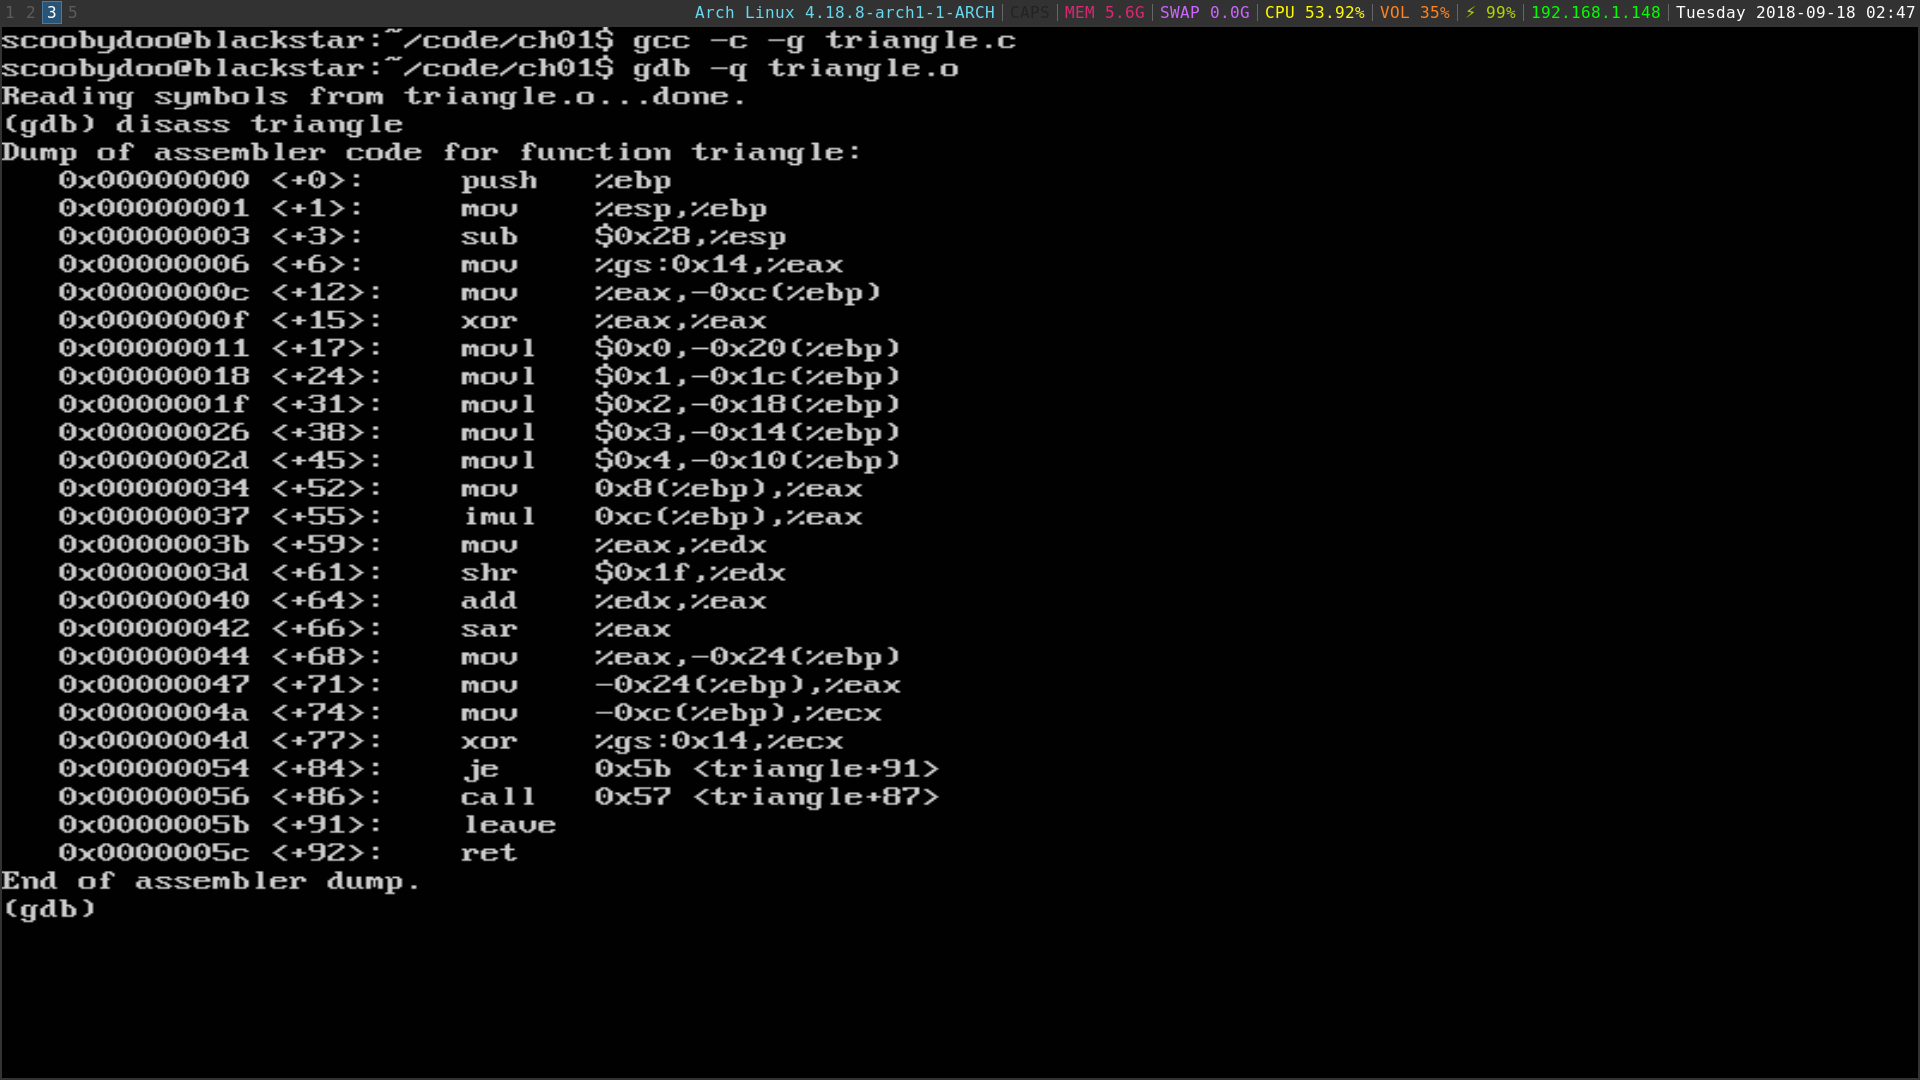
\includegraphics[width=15cm, height=7cm]{triangle_disass.png}
  \caption{Compiling (without linking) then disassembling triangle.c}
\end{figure}
With this example, we can see how a C function actually looks in assembly. First, the \textit{ebp} register (frame pointer) is pushed onto the stack so it can be used within the function then popped off the stack (via the \textit{leave} instruction) after the function returns (a local function variable!). Next, room on the stack is made for local variables (width and height) by subtracting from the \textit{esp} register (stacks grow downwards!). We see the array being initialized and values being stored in it with the \textit{movl} instructions, we see the memory locations are being referenced by offsets with width 4 from \textit{ebp}. We then see the area of the triangle being calculated with instructions like \textit{imul}. This value is stored in the \textit{eax} register, which is used to hold the functions return value. Finally, \textit{ebp} is popped off the stack by the \textit{leave} instruction and the function returns to the caller.

\section{Introduction to stack overflows}
Chapter 2 starts off by explaining what a stack overflow is then gives us a few examples to try out. In this section I will explain how I went about exploiting the \textit{overflow.c} and \textit{serial.c} programs through their buffer overflow vulnerabilities. Throughout this section I will be using Python scripts to help automate and understand the exploits I am carrying out, their will be directories including all the scripts I write and the vulnerable programs they pertain too.

\subsection{Exploiting overflow.c}
To start, we can compile \textit{overflow.c} with the options described in 1ab 1.
\begin{verbatim}
gcc -fno-stack-protector -mpreferred-stack-boundary=2 -z execstack -ggdb
overflow.c -o overflow.out
\end{verbatim}
When running \textit{overflow.c} we see all it does is take user input then display it back to STDOUT. The flaw in this program is that it uses the \textit{gets} function with a fixed sized array, meaning if user input is too long, the buffer will overflow and overwrite memory beyond it. The book holds our hand on how we can dig into this and eventually exploit this bug, I will briefly explain what I did when following the steps in the book. To begin, let's use gdb on the compiled executable so we can poke around:
\begin{verbatim}
gdb -q ./overflow.out
\end{verbatim}
We know the vulnerability is in the \textit{return\_input} function so we can start by disassembling it. We can see the call instruction to the \textit{gets} function, which is where it will ask for user input. To see the effects of our user input (especially when our input is larger than the buffer size) we can put a breakpoint right on the \textit{gets} function and another one after it on the \textit{ret} instruction (just before we return execution to the main function). We can then run our code, which will go until our first breakpoint is hit, as shown in Figure 2 below.
\begin{figure}[H]
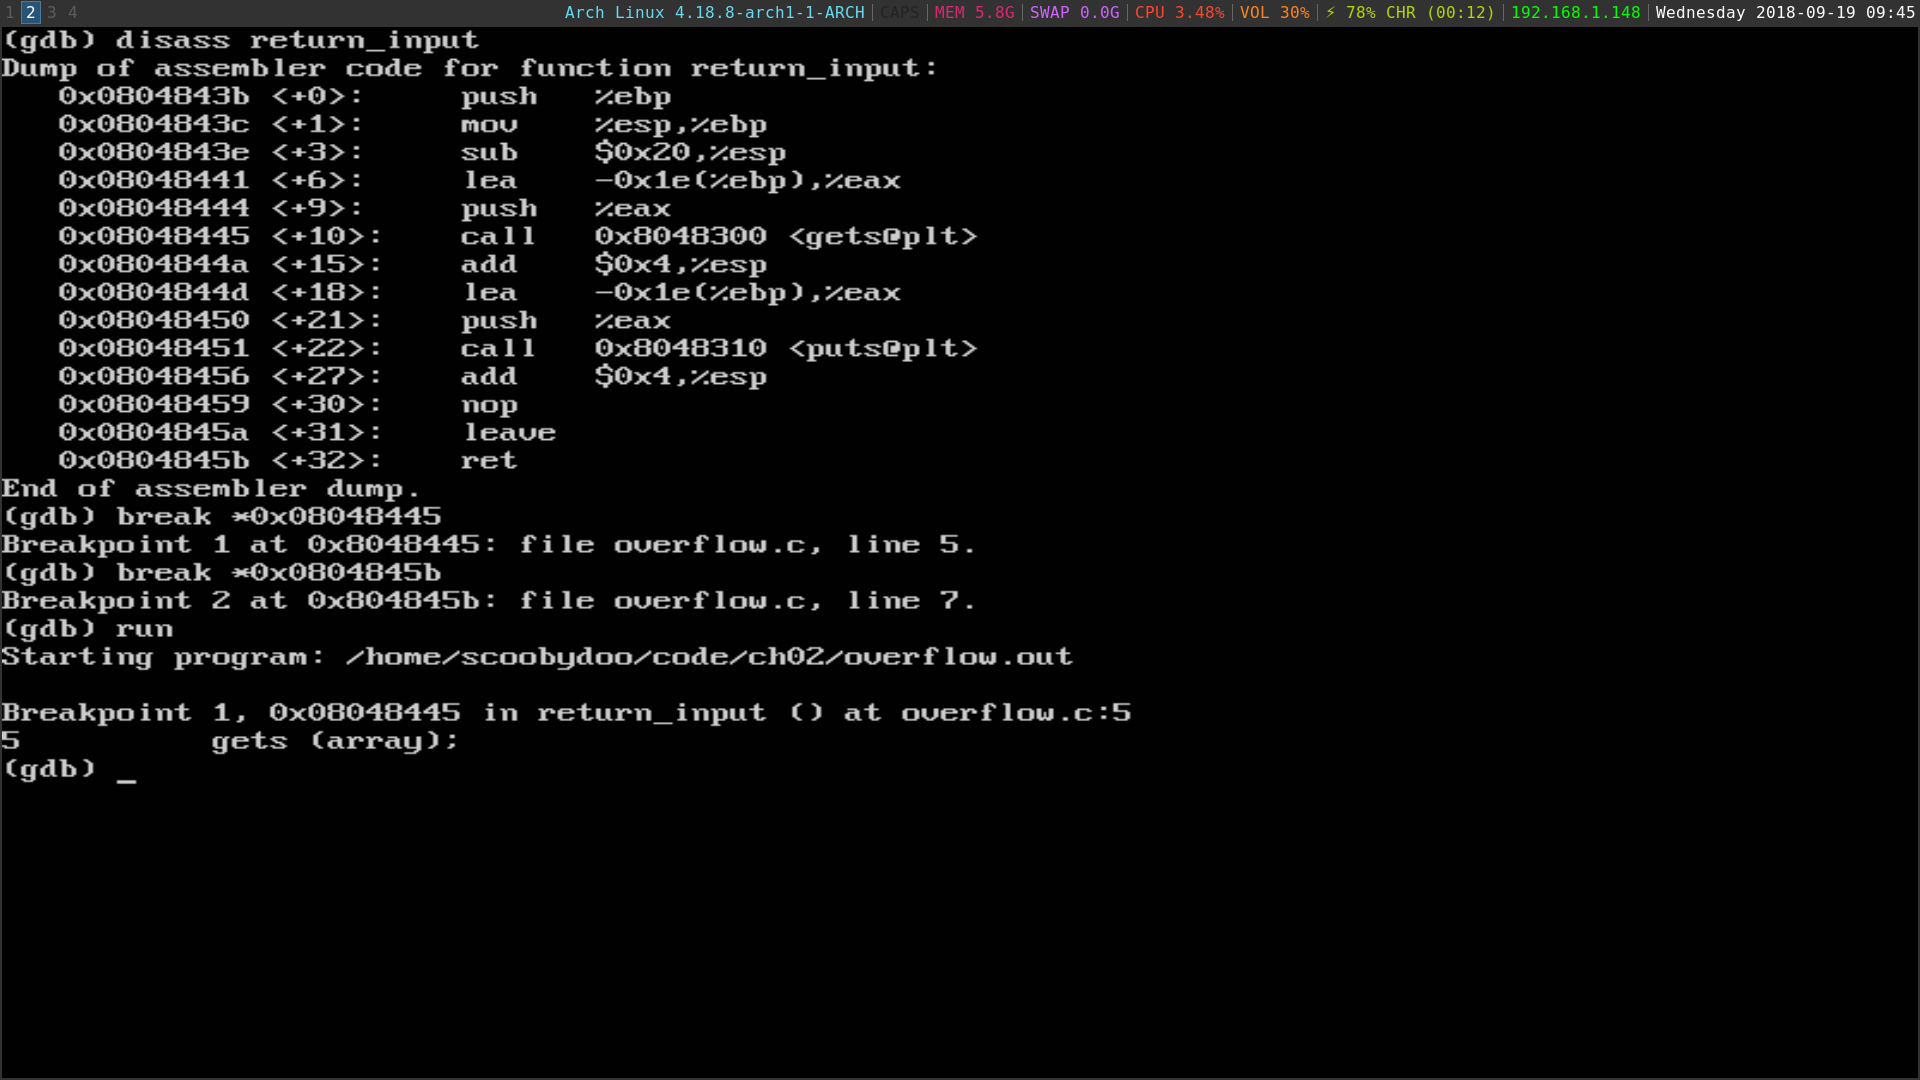
\includegraphics[width=15cm, height=9cm]{overflow1.png}
  \caption{Disassembly of the return\_input function in overflow.c}
\end{figure}
Our goal is to see the effect of user input on our registers, we know after we type our input and move onto our next breakpoint the function will return by referencing the address stored in the \textit{EIP} register. By disassembling main we see the next instruction after returning (what \textit{EIP} will be pointing to) is at address \textit{0x08048465}, this value is also shown on the third row of values when printing the first 20 values beyond the current \textit{ESP} address. Finally, if we give user input that is too long as shown below in Figure 3, we notice that the value stored in \textit{EIP} has now been overwritten with the character's D (hexadecimal 0x44) due to a buffer overflow.
\begin{figure}[H]
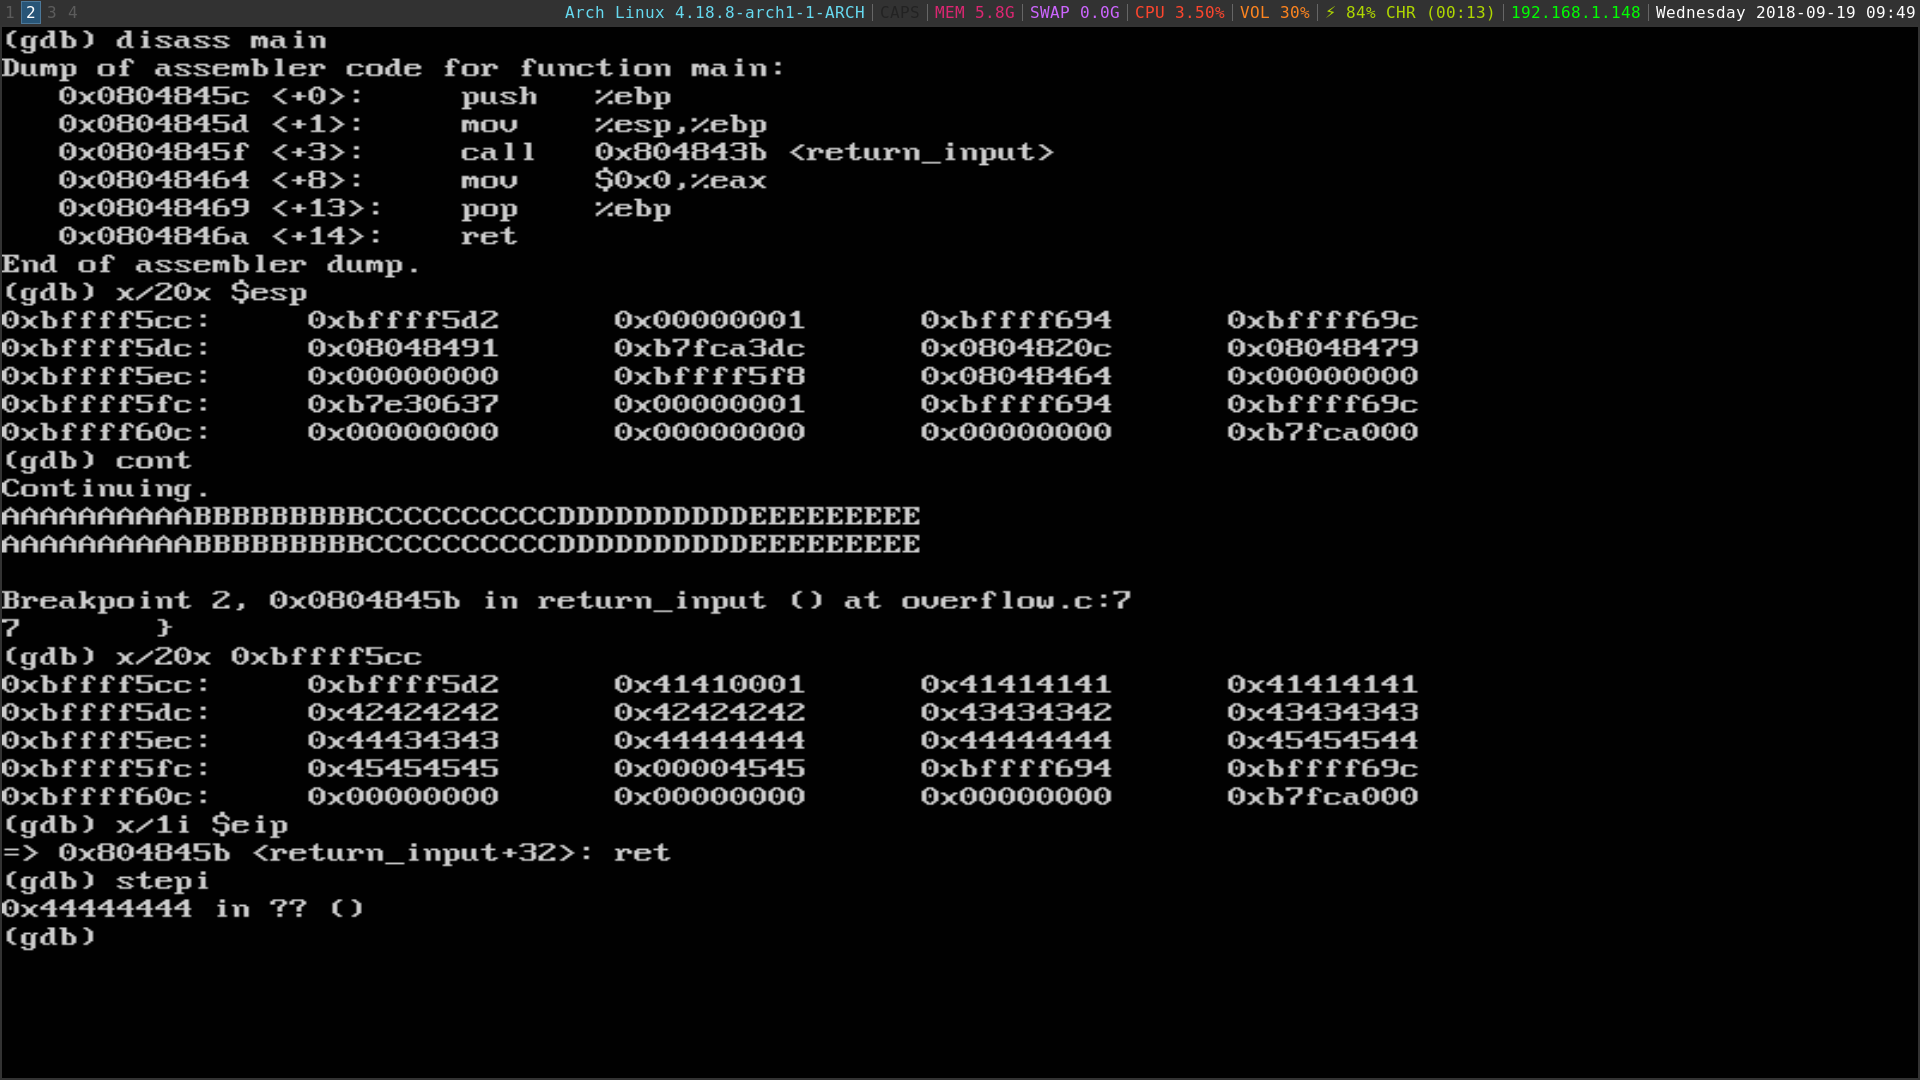
\includegraphics[width=15cm, height=8.5cm]{overflow2.png}
  \caption{Finding the right amount of padding to overwrite/overflow \textit{EIP}}
\end{figure}
In fact, if we count the number of characters, we can see that it took exactly 34 characters before our \textit{EIP} register started getting overwritten by D's. To test this theory, the book recommends trying to store the address of the \textit{return\_input} function to see if we can get \textit{EIP} (the return address) to call \textit{return\_input} for a second time. We can do this by putting the memory address of \textit{return\_input} at the end of our 34 bit padding. Looking back at Figure 3, we see the address of \textit{return\_input} is \textit{0x0804845f} or \verb|\x5f\x84\x04\x08| as little endian escaped bytes.\\

To carry out this exploit, a Python script called \textit{exploit.py} was written, please refer to it for how the exploits were carried out for this section as well as section 3.2.
\subsection{Exploiting serial.c}
This is very similar to the above example, this time around we want to try and trick the program into thinking we put in a valid serial number by exploting a buffer overflow. Instead of looking for the exact amount of padding we need, we can make an estimate then use \textit{exploit.py} to try multiple values for us. This saves a huge amount of effort and is very easy to carry out. First, compile \textit{serial.c}:
\begin{verbatim}
gcc -fno-stack-protector -mpreferred-stack-boundary=2 -z execstack -ggdb
serial.c -o serial.out
\end{verbatim}
We can then use gdb to disassemble the main function to find the address we want \textit{EIP} to point to. Shown in Figure 4, the address we want to jump to is \textit{0x08048601} (the \textit{do\_valid\_stuff} function).
\begin{figure}[H]
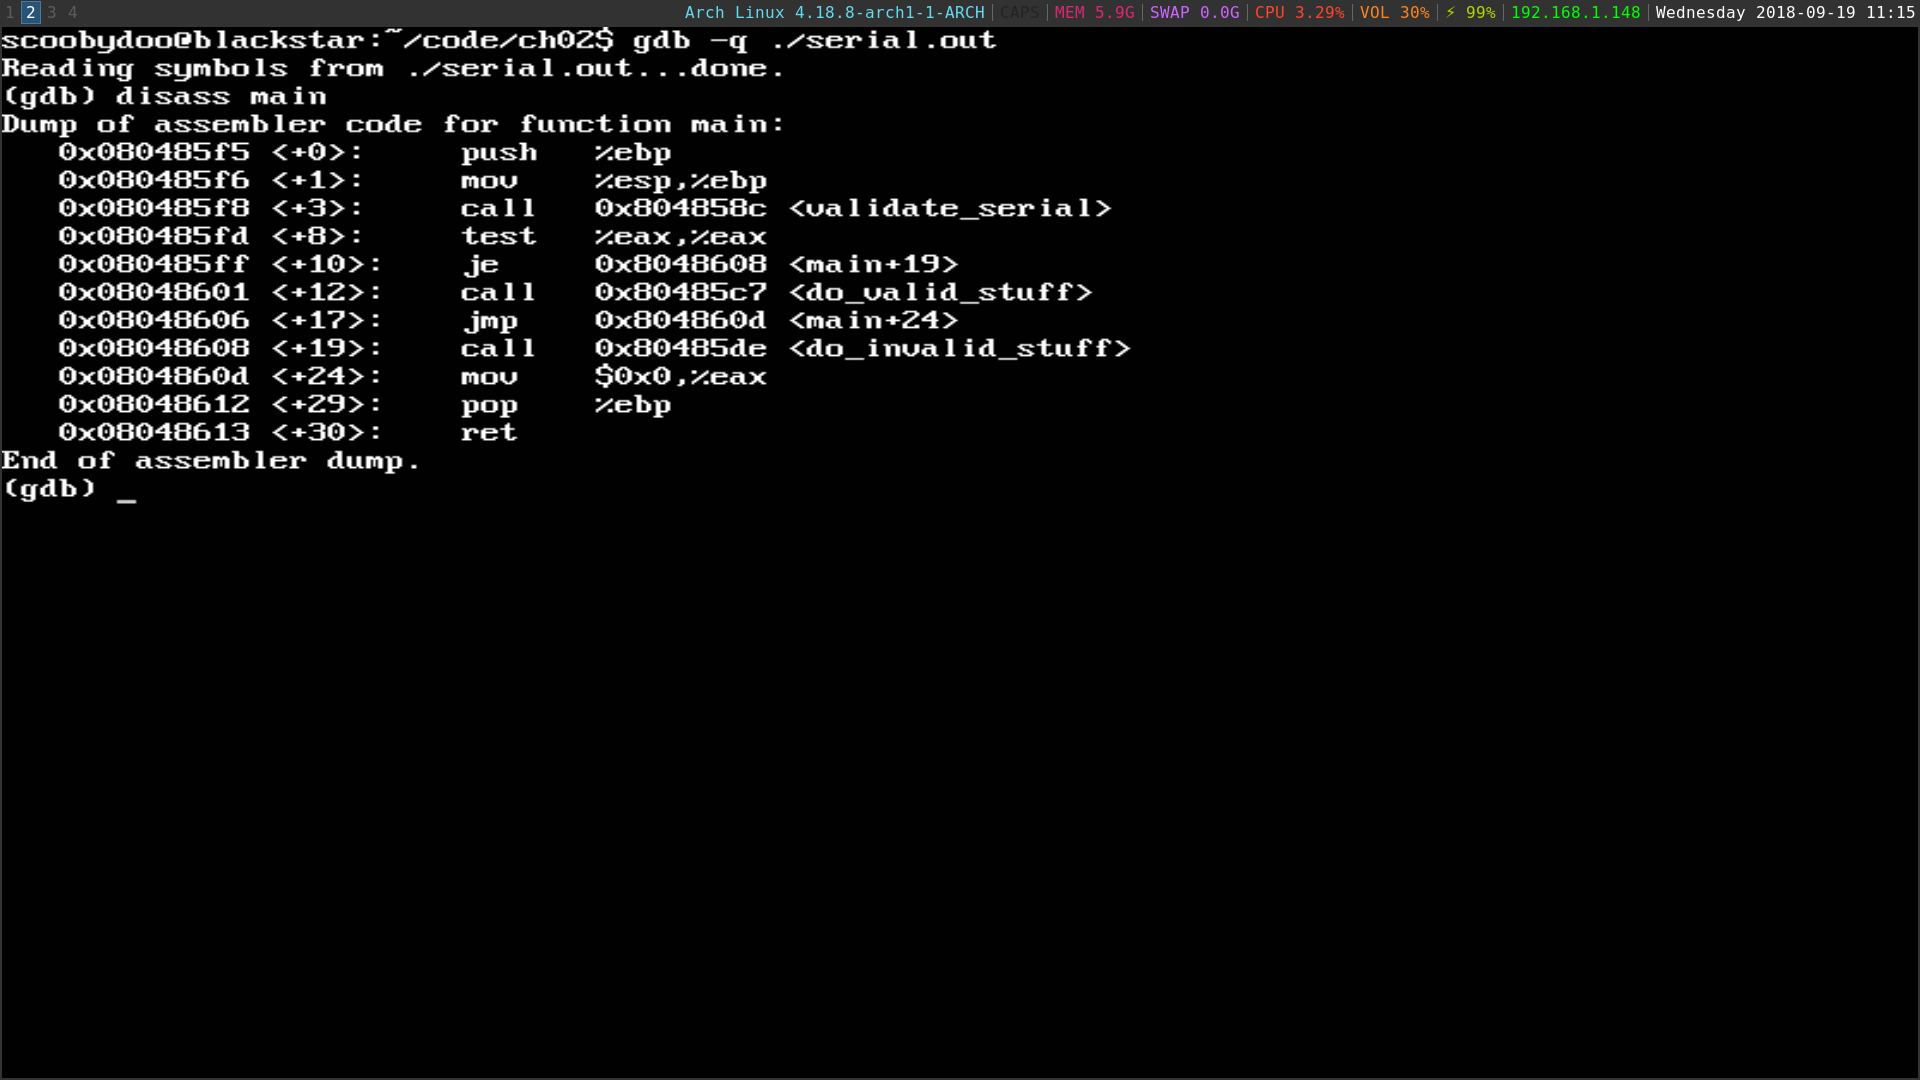
\includegraphics[width=15cm, height=9cm]{serial1.png}
  \caption{Finding the right amount of padding to overwrite/overflow \textit{EIP}}
\end{figure}
We can use the function in \textit{exploit.py} and a simple loop to find the correct padding to overwrite \textit{EIP} successfully, shown below in Figure 5.
\begin{figure}[H]
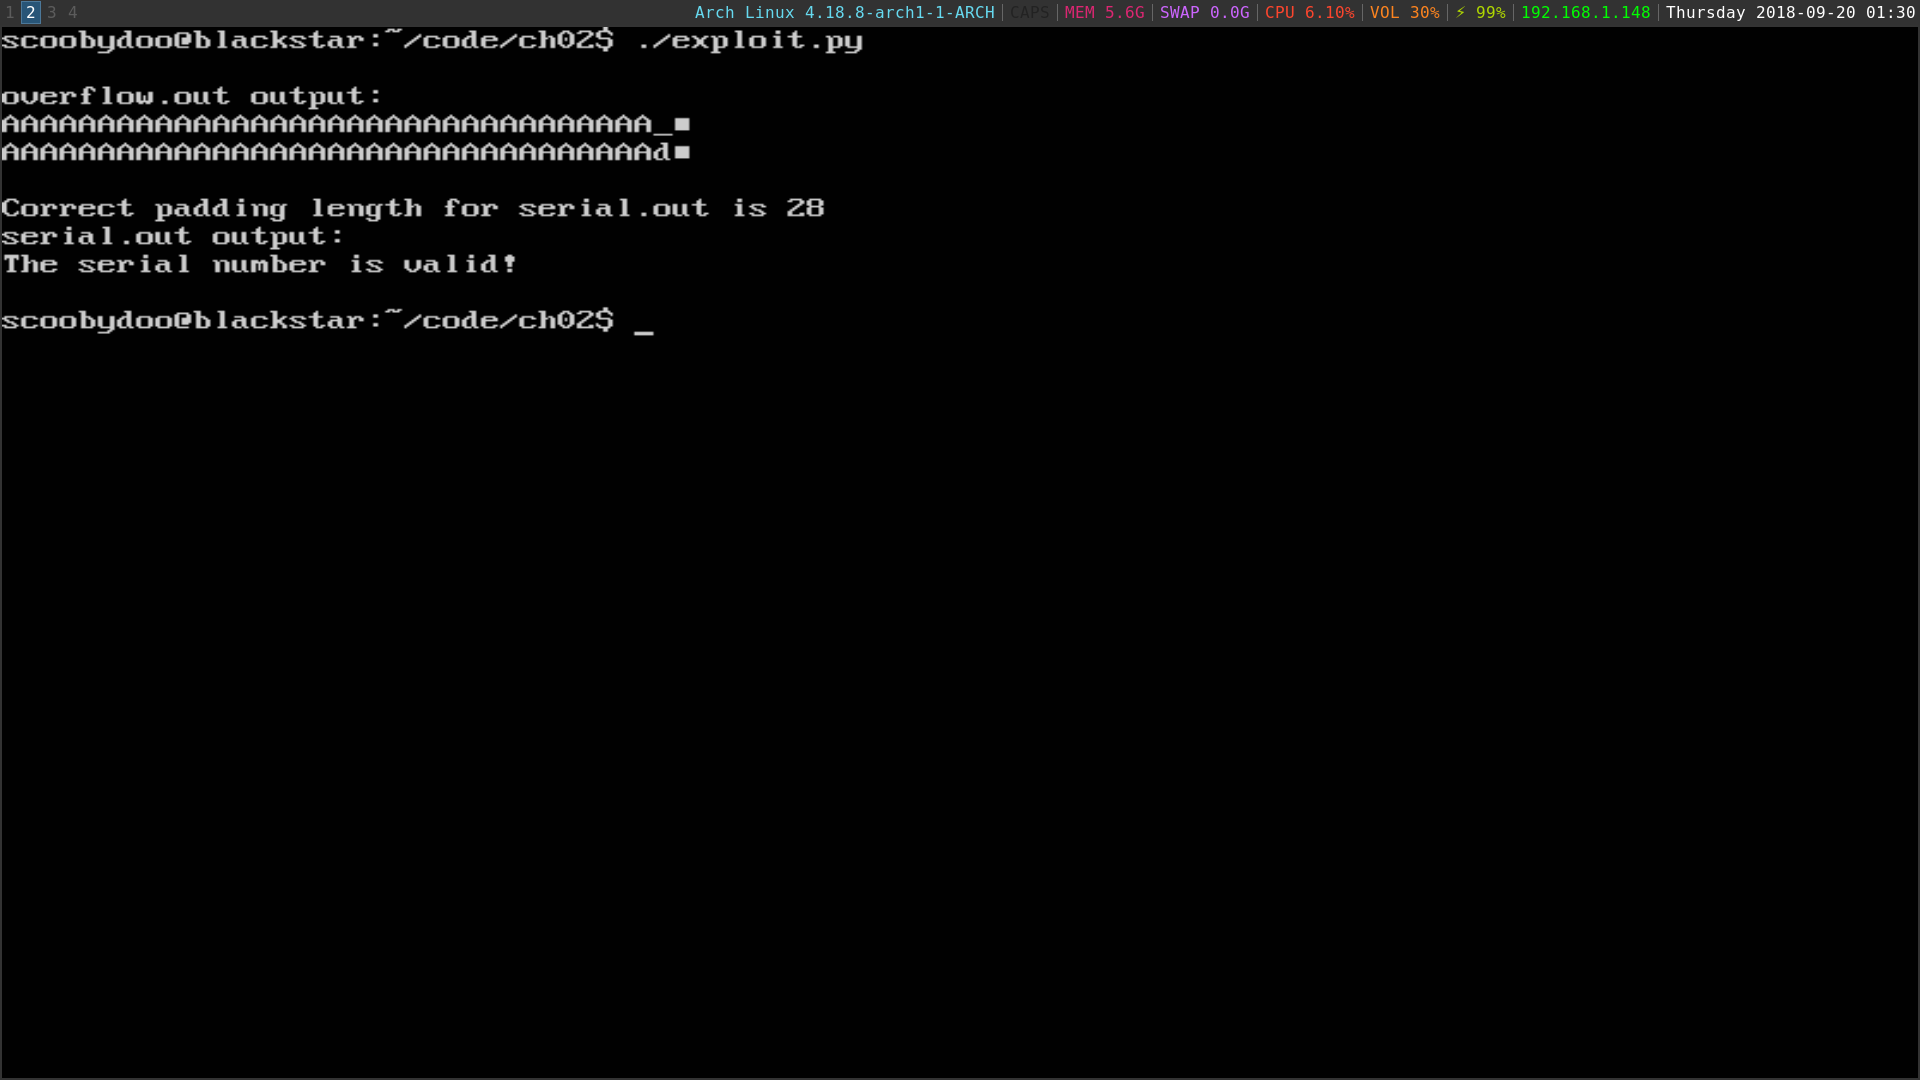
\includegraphics[width=15cm, height=9cm]{exploit_py.png}
  \caption{Bruteforcing the correct amount of padding to overwrite/overflow \textit{EIP}}
\end{figure}

\newpage
\section{Fixing the security flaws}
\subsection{Fixing overflow.c}
The exploitable piece of code in \textit{overflow.c} is the \textit{gets} function. Using the standard library function \textit{gets} is now considered bad practice (reasons why shown above), it is now much safer to use the \textit{fgets} function. This function makes sure you specify the size of the buffer you are storing data into. To fix \textit{overflow.c} simply replace \textit{gets} with a proper call of \textit{fgets}:
\begin{verbatim}
fgets(array, sizeof(array), stdin);
\end{verbatim}

\subsection{Fixing serial.c}
Fixing \textit{serial.c} works in the same way as fixing \textit{overflow.c} with one minor addition. In \textit{serial.c} the \textit{fscanf} function is used, which suffers the same bound checking problem as \textit{gets}. This means we can fix the problem in the same way by replacing \textit{fscanf} with \textit{fgets}, but the problem with this is, \textit{fgets} adds a newline character ('\textbackslash n') to the end of the buffer, always making our serial number invalid. To fix this we can still call \textit{fgets} but use the function \textit{strcspn} to span the buffer and replace the newline character with a null value [3]:
\begin{verbatim}
fgets(serial, sizeof(serial), stdin);
serial(strcspn(serial, "\n")) = 0;
\end{verbatim}

\section{Conclusions}
We now know a little more about x86 assembly as well as the basics of what a stack overflow is and how to exploit them. We have created a simple Python script to help exploit stack overflows in a more automated fashion and can extend it in the next labs, when we learn to create and execute useful shellcode.

\section{References}

\begin{enumerate}
  \item\href{https://docs.python.org/3/library/subprocess.html#subprocess.Popen}{\textbf{Python subprocess documentation}}
  \newline\indent https://docs.python.org/3/library/subprocess.html\#subprocess.Popen

  \item\href{http://phrack.org/issues/49/14.html#article}{\textbf{Smashing The Stack For Fun And Profit}}
  \newline\indent http://phrack.org/issues/49/14.html\#article

  \item\href{https://stackoverflow.com/questions/2693776/removing-trailing-newline-character-from-fgets-input}{\textbf{Removing trailing newline character from fgets() input}}
  \newline\indent https://stackoverflow.com/questions/2693776/removing-trailing-newline-character-from-fgets-input
\end{enumerate}

\end{document}
